% Generated by Sphinx.
\def\sphinxdocclass{article}
\documentclass[a4paper,10pt,french]{sphinxhowto}
\usepackage[utf8]{inputenc}
\DeclareUnicodeCharacter{00A0}{\nobreakspace}
\usepackage{cmap}
\usepackage[T1]{fontenc}
\usepackage{babel}
\usepackage{times}
\usepackage[Sonny]{fncychap}
\usepackage{longtable}
\usepackage{sphinx}
\usepackage{multirow}

\addto\captionsfrench{\renewcommand{\figurename}{Fig. }}
\addto\captionsfrench{\renewcommand{\tablename}{Tableau }}
\floatname{literal-block}{Code source }



\title{CIR-2015 : Photogrammetrie}
\date{18 July 2016}
\release{}
\author{la maison - Paris}
\newcommand{\sphinxlogo}{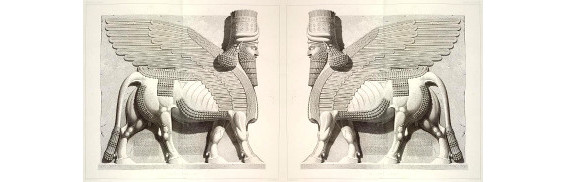
\includegraphics{Lamassu_small.jpg}\par}
\renewcommand{\releasename}{}
\makeindex

\makeatletter
\def\PYG@reset{\let\PYG@it=\relax \let\PYG@bf=\relax%
    \let\PYG@ul=\relax \let\PYG@tc=\relax%
    \let\PYG@bc=\relax \let\PYG@ff=\relax}
\def\PYG@tok#1{\csname PYG@tok@#1\endcsname}
\def\PYG@toks#1+{\ifx\relax#1\empty\else%
    \PYG@tok{#1}\expandafter\PYG@toks\fi}
\def\PYG@do#1{\PYG@bc{\PYG@tc{\PYG@ul{%
    \PYG@it{\PYG@bf{\PYG@ff{#1}}}}}}}
\def\PYG#1#2{\PYG@reset\PYG@toks#1+\relax+\PYG@do{#2}}

\expandafter\def\csname PYG@tok@gd\endcsname{\def\PYG@tc##1{\textcolor[rgb]{0.63,0.00,0.00}{##1}}}
\expandafter\def\csname PYG@tok@gu\endcsname{\let\PYG@bf=\textbf\def\PYG@tc##1{\textcolor[rgb]{0.50,0.00,0.50}{##1}}}
\expandafter\def\csname PYG@tok@gt\endcsname{\def\PYG@tc##1{\textcolor[rgb]{0.00,0.27,0.87}{##1}}}
\expandafter\def\csname PYG@tok@gs\endcsname{\let\PYG@bf=\textbf}
\expandafter\def\csname PYG@tok@gr\endcsname{\def\PYG@tc##1{\textcolor[rgb]{1.00,0.00,0.00}{##1}}}
\expandafter\def\csname PYG@tok@cm\endcsname{\let\PYG@it=\textit\def\PYG@tc##1{\textcolor[rgb]{0.25,0.50,0.56}{##1}}}
\expandafter\def\csname PYG@tok@vg\endcsname{\def\PYG@tc##1{\textcolor[rgb]{0.73,0.38,0.84}{##1}}}
\expandafter\def\csname PYG@tok@m\endcsname{\def\PYG@tc##1{\textcolor[rgb]{0.13,0.50,0.31}{##1}}}
\expandafter\def\csname PYG@tok@mh\endcsname{\def\PYG@tc##1{\textcolor[rgb]{0.13,0.50,0.31}{##1}}}
\expandafter\def\csname PYG@tok@cs\endcsname{\def\PYG@tc##1{\textcolor[rgb]{0.25,0.50,0.56}{##1}}\def\PYG@bc##1{\setlength{\fboxsep}{0pt}\colorbox[rgb]{1.00,0.94,0.94}{\strut ##1}}}
\expandafter\def\csname PYG@tok@ge\endcsname{\let\PYG@it=\textit}
\expandafter\def\csname PYG@tok@vc\endcsname{\def\PYG@tc##1{\textcolor[rgb]{0.73,0.38,0.84}{##1}}}
\expandafter\def\csname PYG@tok@il\endcsname{\def\PYG@tc##1{\textcolor[rgb]{0.13,0.50,0.31}{##1}}}
\expandafter\def\csname PYG@tok@go\endcsname{\def\PYG@tc##1{\textcolor[rgb]{0.20,0.20,0.20}{##1}}}
\expandafter\def\csname PYG@tok@cp\endcsname{\def\PYG@tc##1{\textcolor[rgb]{0.00,0.44,0.13}{##1}}}
\expandafter\def\csname PYG@tok@gi\endcsname{\def\PYG@tc##1{\textcolor[rgb]{0.00,0.63,0.00}{##1}}}
\expandafter\def\csname PYG@tok@gh\endcsname{\let\PYG@bf=\textbf\def\PYG@tc##1{\textcolor[rgb]{0.00,0.00,0.50}{##1}}}
\expandafter\def\csname PYG@tok@ni\endcsname{\let\PYG@bf=\textbf\def\PYG@tc##1{\textcolor[rgb]{0.84,0.33,0.22}{##1}}}
\expandafter\def\csname PYG@tok@nl\endcsname{\let\PYG@bf=\textbf\def\PYG@tc##1{\textcolor[rgb]{0.00,0.13,0.44}{##1}}}
\expandafter\def\csname PYG@tok@nn\endcsname{\let\PYG@bf=\textbf\def\PYG@tc##1{\textcolor[rgb]{0.05,0.52,0.71}{##1}}}
\expandafter\def\csname PYG@tok@no\endcsname{\def\PYG@tc##1{\textcolor[rgb]{0.38,0.68,0.84}{##1}}}
\expandafter\def\csname PYG@tok@na\endcsname{\def\PYG@tc##1{\textcolor[rgb]{0.25,0.44,0.63}{##1}}}
\expandafter\def\csname PYG@tok@nb\endcsname{\def\PYG@tc##1{\textcolor[rgb]{0.00,0.44,0.13}{##1}}}
\expandafter\def\csname PYG@tok@nc\endcsname{\let\PYG@bf=\textbf\def\PYG@tc##1{\textcolor[rgb]{0.05,0.52,0.71}{##1}}}
\expandafter\def\csname PYG@tok@nd\endcsname{\let\PYG@bf=\textbf\def\PYG@tc##1{\textcolor[rgb]{0.33,0.33,0.33}{##1}}}
\expandafter\def\csname PYG@tok@ne\endcsname{\def\PYG@tc##1{\textcolor[rgb]{0.00,0.44,0.13}{##1}}}
\expandafter\def\csname PYG@tok@nf\endcsname{\def\PYG@tc##1{\textcolor[rgb]{0.02,0.16,0.49}{##1}}}
\expandafter\def\csname PYG@tok@si\endcsname{\let\PYG@it=\textit\def\PYG@tc##1{\textcolor[rgb]{0.44,0.63,0.82}{##1}}}
\expandafter\def\csname PYG@tok@s2\endcsname{\def\PYG@tc##1{\textcolor[rgb]{0.25,0.44,0.63}{##1}}}
\expandafter\def\csname PYG@tok@vi\endcsname{\def\PYG@tc##1{\textcolor[rgb]{0.73,0.38,0.84}{##1}}}
\expandafter\def\csname PYG@tok@nt\endcsname{\let\PYG@bf=\textbf\def\PYG@tc##1{\textcolor[rgb]{0.02,0.16,0.45}{##1}}}
\expandafter\def\csname PYG@tok@nv\endcsname{\def\PYG@tc##1{\textcolor[rgb]{0.73,0.38,0.84}{##1}}}
\expandafter\def\csname PYG@tok@s1\endcsname{\def\PYG@tc##1{\textcolor[rgb]{0.25,0.44,0.63}{##1}}}
\expandafter\def\csname PYG@tok@gp\endcsname{\let\PYG@bf=\textbf\def\PYG@tc##1{\textcolor[rgb]{0.78,0.36,0.04}{##1}}}
\expandafter\def\csname PYG@tok@sh\endcsname{\def\PYG@tc##1{\textcolor[rgb]{0.25,0.44,0.63}{##1}}}
\expandafter\def\csname PYG@tok@ow\endcsname{\let\PYG@bf=\textbf\def\PYG@tc##1{\textcolor[rgb]{0.00,0.44,0.13}{##1}}}
\expandafter\def\csname PYG@tok@sx\endcsname{\def\PYG@tc##1{\textcolor[rgb]{0.78,0.36,0.04}{##1}}}
\expandafter\def\csname PYG@tok@bp\endcsname{\def\PYG@tc##1{\textcolor[rgb]{0.00,0.44,0.13}{##1}}}
\expandafter\def\csname PYG@tok@c1\endcsname{\let\PYG@it=\textit\def\PYG@tc##1{\textcolor[rgb]{0.25,0.50,0.56}{##1}}}
\expandafter\def\csname PYG@tok@kc\endcsname{\let\PYG@bf=\textbf\def\PYG@tc##1{\textcolor[rgb]{0.00,0.44,0.13}{##1}}}
\expandafter\def\csname PYG@tok@c\endcsname{\let\PYG@it=\textit\def\PYG@tc##1{\textcolor[rgb]{0.25,0.50,0.56}{##1}}}
\expandafter\def\csname PYG@tok@mf\endcsname{\def\PYG@tc##1{\textcolor[rgb]{0.13,0.50,0.31}{##1}}}
\expandafter\def\csname PYG@tok@err\endcsname{\def\PYG@bc##1{\setlength{\fboxsep}{0pt}\fcolorbox[rgb]{1.00,0.00,0.00}{1,1,1}{\strut ##1}}}
\expandafter\def\csname PYG@tok@mb\endcsname{\def\PYG@tc##1{\textcolor[rgb]{0.13,0.50,0.31}{##1}}}
\expandafter\def\csname PYG@tok@ss\endcsname{\def\PYG@tc##1{\textcolor[rgb]{0.32,0.47,0.09}{##1}}}
\expandafter\def\csname PYG@tok@sr\endcsname{\def\PYG@tc##1{\textcolor[rgb]{0.14,0.33,0.53}{##1}}}
\expandafter\def\csname PYG@tok@mo\endcsname{\def\PYG@tc##1{\textcolor[rgb]{0.13,0.50,0.31}{##1}}}
\expandafter\def\csname PYG@tok@kd\endcsname{\let\PYG@bf=\textbf\def\PYG@tc##1{\textcolor[rgb]{0.00,0.44,0.13}{##1}}}
\expandafter\def\csname PYG@tok@mi\endcsname{\def\PYG@tc##1{\textcolor[rgb]{0.13,0.50,0.31}{##1}}}
\expandafter\def\csname PYG@tok@kn\endcsname{\let\PYG@bf=\textbf\def\PYG@tc##1{\textcolor[rgb]{0.00,0.44,0.13}{##1}}}
\expandafter\def\csname PYG@tok@o\endcsname{\def\PYG@tc##1{\textcolor[rgb]{0.40,0.40,0.40}{##1}}}
\expandafter\def\csname PYG@tok@kr\endcsname{\let\PYG@bf=\textbf\def\PYG@tc##1{\textcolor[rgb]{0.00,0.44,0.13}{##1}}}
\expandafter\def\csname PYG@tok@s\endcsname{\def\PYG@tc##1{\textcolor[rgb]{0.25,0.44,0.63}{##1}}}
\expandafter\def\csname PYG@tok@kp\endcsname{\def\PYG@tc##1{\textcolor[rgb]{0.00,0.44,0.13}{##1}}}
\expandafter\def\csname PYG@tok@w\endcsname{\def\PYG@tc##1{\textcolor[rgb]{0.73,0.73,0.73}{##1}}}
\expandafter\def\csname PYG@tok@kt\endcsname{\def\PYG@tc##1{\textcolor[rgb]{0.56,0.13,0.00}{##1}}}
\expandafter\def\csname PYG@tok@sc\endcsname{\def\PYG@tc##1{\textcolor[rgb]{0.25,0.44,0.63}{##1}}}
\expandafter\def\csname PYG@tok@sb\endcsname{\def\PYG@tc##1{\textcolor[rgb]{0.25,0.44,0.63}{##1}}}
\expandafter\def\csname PYG@tok@k\endcsname{\let\PYG@bf=\textbf\def\PYG@tc##1{\textcolor[rgb]{0.00,0.44,0.13}{##1}}}
\expandafter\def\csname PYG@tok@se\endcsname{\let\PYG@bf=\textbf\def\PYG@tc##1{\textcolor[rgb]{0.25,0.44,0.63}{##1}}}
\expandafter\def\csname PYG@tok@sd\endcsname{\let\PYG@it=\textit\def\PYG@tc##1{\textcolor[rgb]{0.25,0.44,0.63}{##1}}}

\def\PYGZbs{\char`\\}
\def\PYGZus{\char`\_}
\def\PYGZob{\char`\{}
\def\PYGZcb{\char`\}}
\def\PYGZca{\char`\^}
\def\PYGZam{\char`\&}
\def\PYGZlt{\char`\<}
\def\PYGZgt{\char`\>}
\def\PYGZsh{\char`\#}
\def\PYGZpc{\char`\%}
\def\PYGZdl{\char`\$}
\def\PYGZhy{\char`\-}
\def\PYGZsq{\char`\'}
\def\PYGZdq{\char`\"}
\def\PYGZti{\char`\~}
% for compatibility with earlier versions
\def\PYGZat{@}
\def\PYGZlb{[}
\def\PYGZrb{]}
\makeatother

\renewcommand\PYGZsq{\textquotesingle}

\begin{document}

\maketitle
\tableofcontents
\phantomsection\label{index::doc}



\section{Introduction}
\label{introduction:introduction}\label{introduction:les-dernieres-pierres-de-mesopotamie}\label{introduction::doc}
{\hfill\scalebox{0.800000}{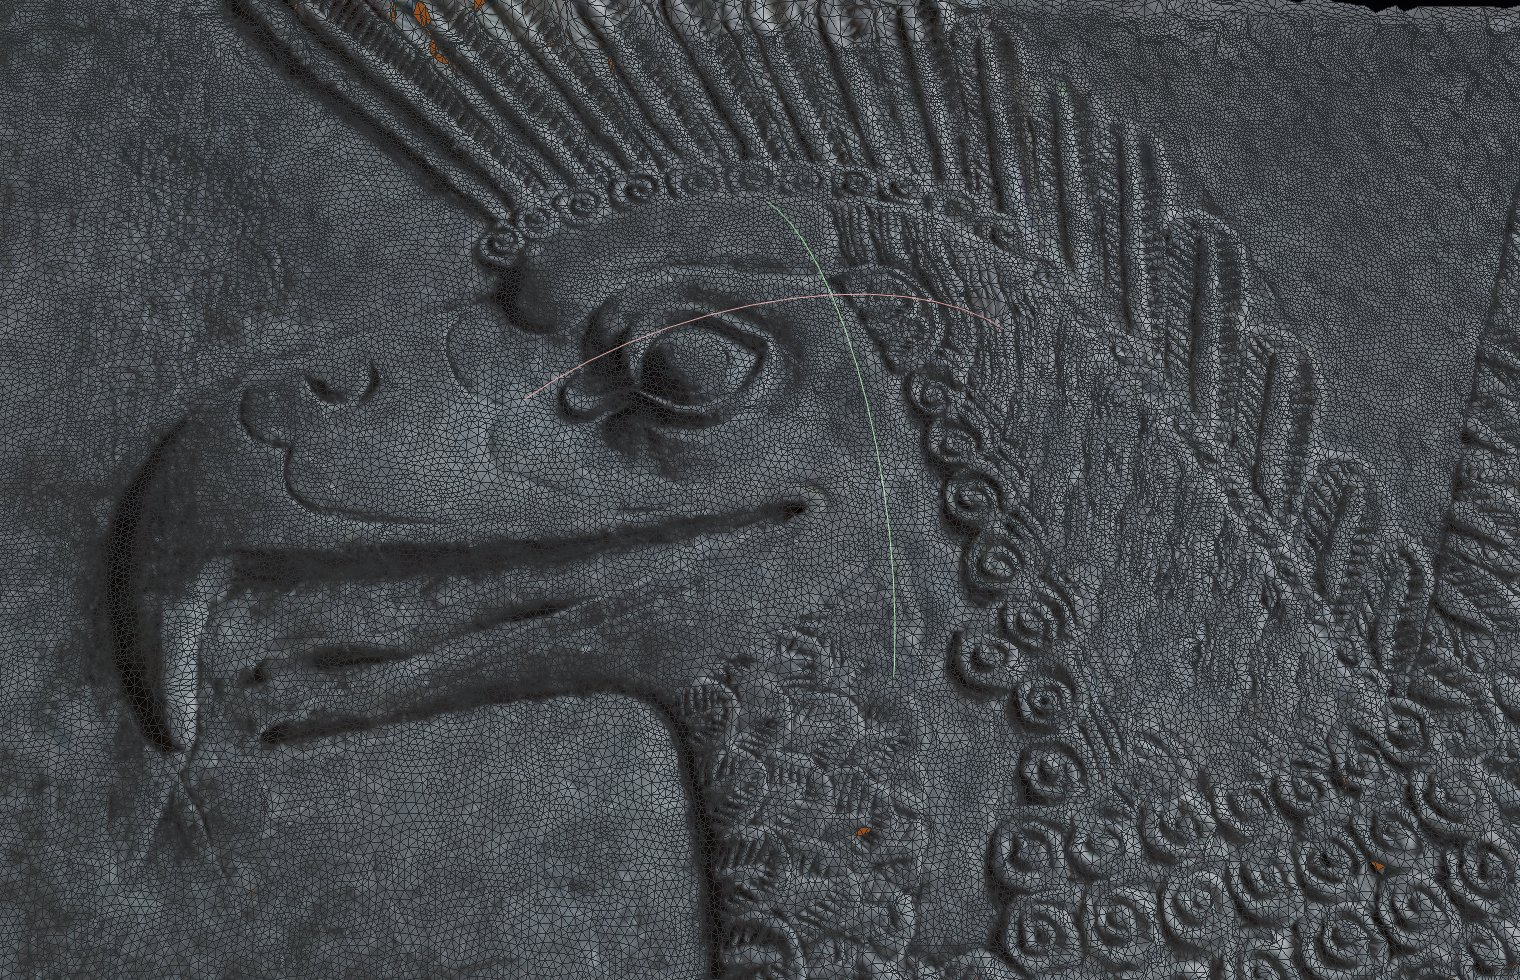
\includegraphics{mysnap73.jpg}}\hfill}

Ce document décrit de manière détaillée les développements que nous souhaitons utiliser pour modéliser et reproduire des modeles 3D a partir de photos.

Ce document est illustré avec des images empruntées a un projet de documentaire sur les les vestiges de la civilisation Assyrienne pour Arte.

Le principe général consiste a collecter sur Internet des images de sculptures ou de bas-relief puis a utiliser des techniques de photogrammétrie pour recréer un modèle numérique 3D.

La reconstruction photogrammétrique est basée sur l’enchaînement de 2 techniques:


\subsection{\textbf{Structure from motion (Sfm)}}
\label{introduction:structure-from-motion-sfm}\begin{quote}

cette première phase permet de retrouver les paramètres intrinsèques (focale,distorsion) ainsi que les paramètres extrinsèques (position,orientation) des cameras ayant servi a prendre les photos originales.Il génère aussi un nuage de points 3D décrivant de manière sommaire l'objet observe (sparse point cloud).Il comporte en général plusieurs centaines voire plusieurs milliers de points.
\end{quote}


\subsection{\textbf{Multi view Stereo (Mvs)}}
\label{introduction:multi-view-stereo-mvs}\begin{quote}

Lors de cette deuxième phase , les résultats obtenus précédemment sont exploités pour générer un nuage de points 3D beaucoup plus dense (dense point cloud).Il est constitue habituellement de plusieurs millions de points.Ces points sont obtenus en analysant les similitudes entre les différentes images.Ce nuage de points est alors utilise pour construire un maillage polygonal de l'objet observé.Au final ce maillage servira de support pour générer une texture 2D combinant les meilleures photographies initiales.
\end{quote}

Le maillage final comporte en général des irrégularités ou des trous.En effet les images sources étant de nature très hétérogènes (conditions d’éclairage et colorimétrie différentes).Les objets observes n'apparaissant pas obligatoirement sous tout les angles possibles.La finalisation des objets se fera manuellement par un artiste 3D dans des logiciels tel que Zbrush (Pixologic) ou 3DCoat.

Les objets obtenus peuvent être extrêmement dense (plusieurs millions de polygones).Afin de pouvoir les manipuler plus aisément dans les logiciels 3D une dernière phase consiste a générer des modèles basse résolution (low-def) et d'y associer des textures représentant le déplacement par rapport a l'objet haute définition (displacement map).La combinaison de ces 2 éléments permet de retrouver la finesse des détails lors du rendu 3D.


\section{Collecte de photos sur Internet}
\label{collection:collecte-de-photos-sur-internet}\label{collection::doc}
Internet permet d’accéder a une masse gigantesque d'images.Afin de pouvoir downloader une collection conséquente d'images nous avons besoin d’accéder a ces recherches par une interface de commandes (cli).

Il existe essentiellement 2 sources de photos accessibles par mot-clef:


\subsection{\textbf{Google Images}}
\label{collection:google-images}\begin{figure}[htbp]
\centering
\capstart

\scalebox{1.000000}{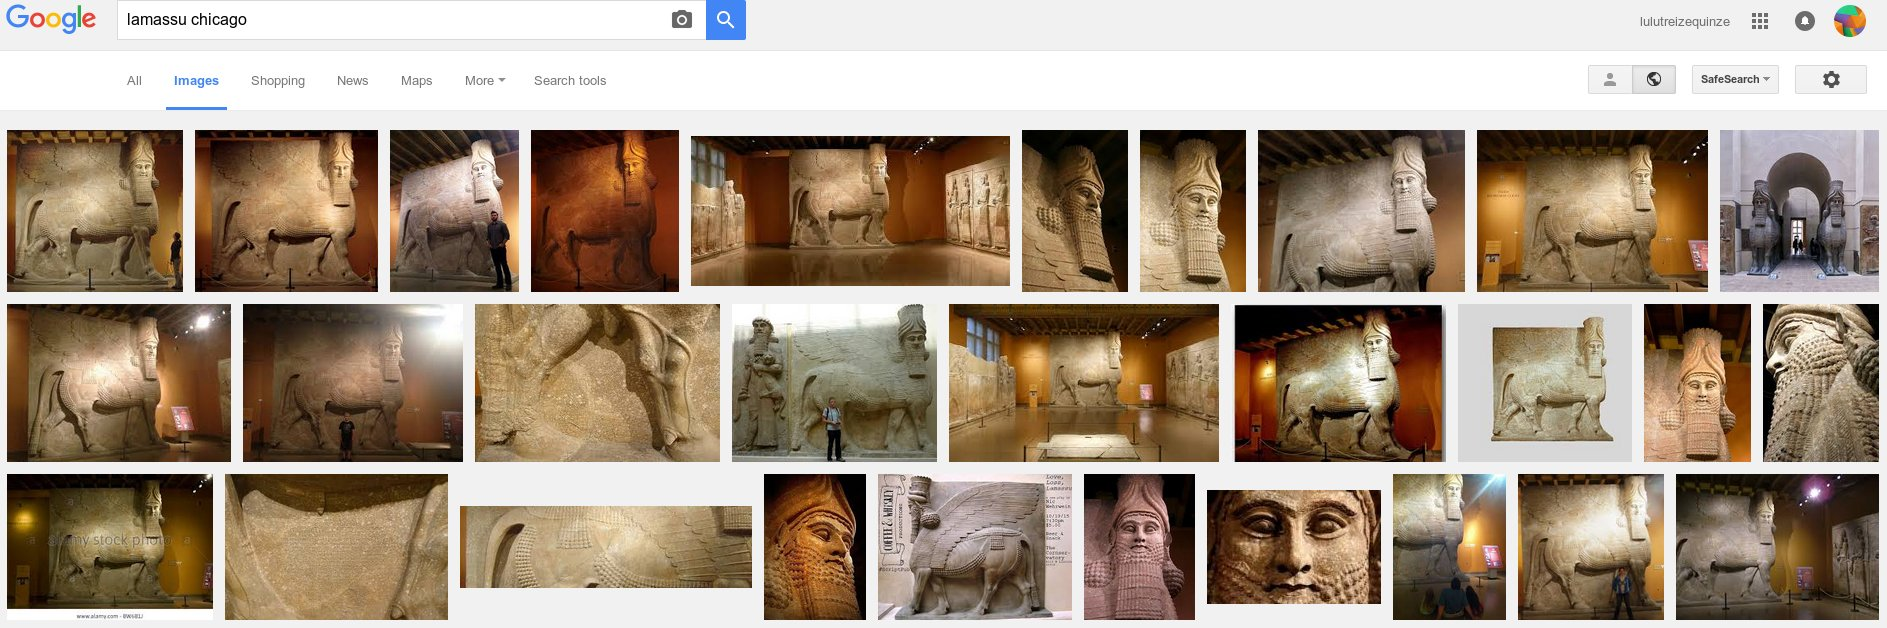
\includegraphics{mysnap5.jpg}}
\caption{exemple de recherche Google image}{\small 
ici un Lamassu Assyrien exposé au musée Oriental de Chicago
}\end{figure}

Google ne propose plus de cli pour downloader automatiquement une sélection d'images par mot clef. Neanmoins en downloadant le contenu html du résultat d'une recherche et en le filtrant on peut récupérer les URL's des images.Nous avons écrit un script en langage Perl permettant de faire cela.Malheureusement Google limite les résultats des recherches a 100 images.Ce qui limite un petit peu les résultats.


\subsection{\textbf{Flickr Images}}
\label{collection:flickr-images}
Flickr (Yahoo) propose une API accessible dans différents langages de programmation.Nous avons choisi le module Perl Flickr::API qui permet d'automatiser la recherche et le téléchargement d'images sur le site de Flickr. Un des grands avantages de Flickr est de donner accès aux images originales des appareils photos et donc a leur informations (MetaData) EXIF.

En effet pour la plupart des algorithmes de StructureFromMotion ces données sont indispensables pour initialiser le processus incrémental de reconstruction des positions de cameras.

La majorité de nos images proviendront donc de Flickr.
\begin{figure}[htbp]
\centering
\capstart

\scalebox{1.000000}{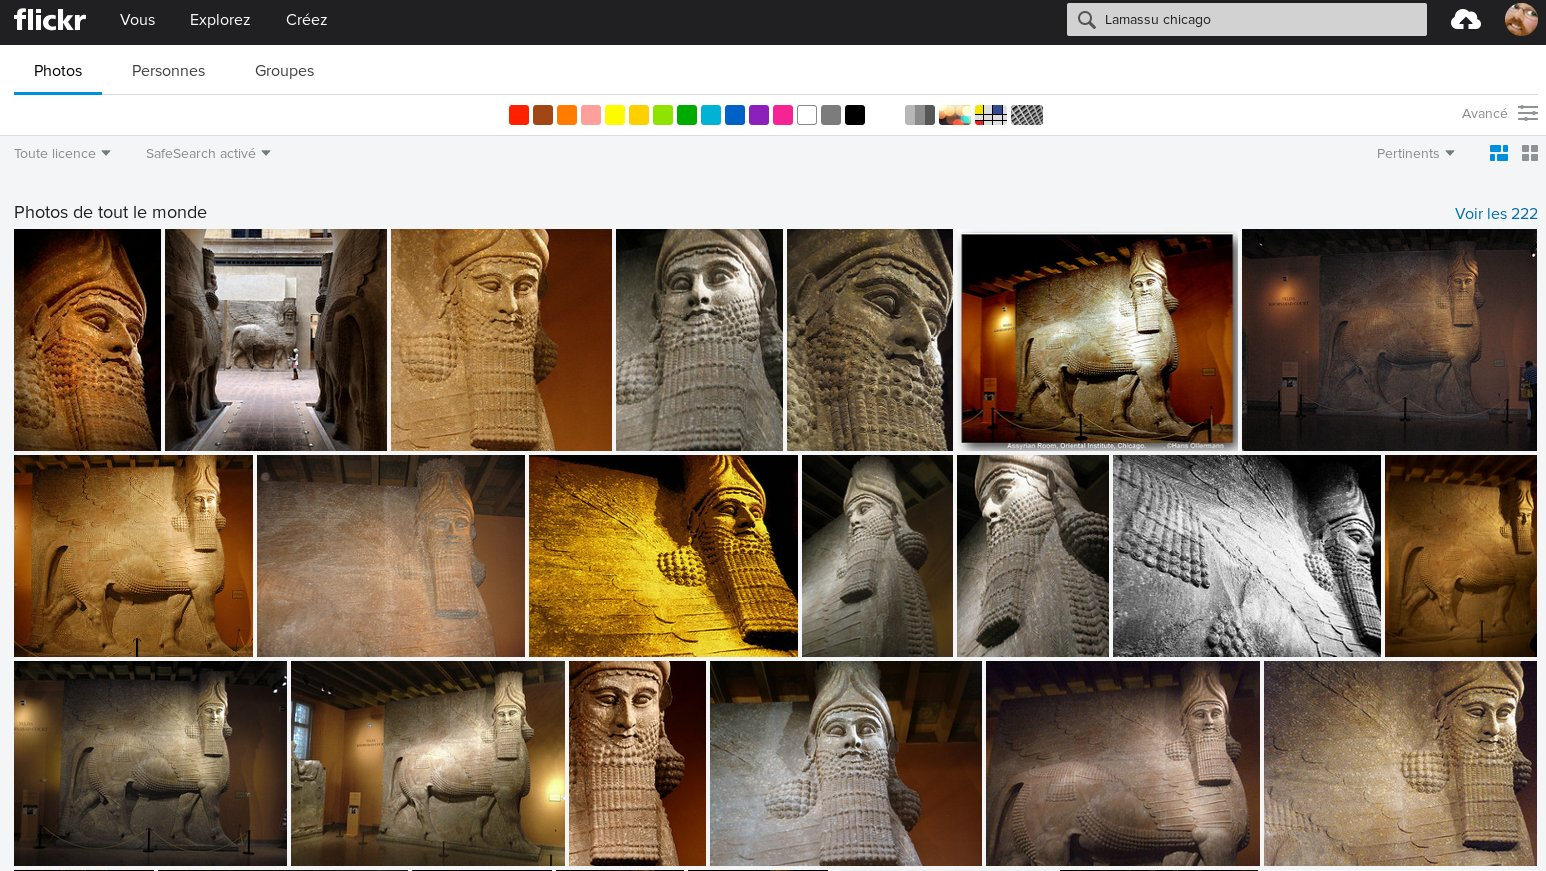
\includegraphics{mysnap4.jpg}}
\caption{exemple de recherche Flickr image}{\small 
Flickr retourne 222 images pour cette recherche
}\end{figure}


\subsection{\textbf{traitement des données EXIFs}}
\label{collection:traitement-des-donnees-exifs}
Les informations contenues dans les données EXIF nous servent a retrouver deux informations fondamentales pour initialiser les valeurs intrinsèques des cameras : la focale et la taille du capteur CMOS ou CCD utilise lors de la prise de vue.La focale est en général inscrite explicitement dans les données EXIFs. Par contre pour retrouver la taille du capteur il est nécessaire d’accéder a deux informations EXIFs : le Modèle et le Type de l'appareil photo.Ces deux paramètres sont en général fourni dans les EXIFs.
\begin{figure}[htbp]
\centering
\capstart

\scalebox{1.000000}{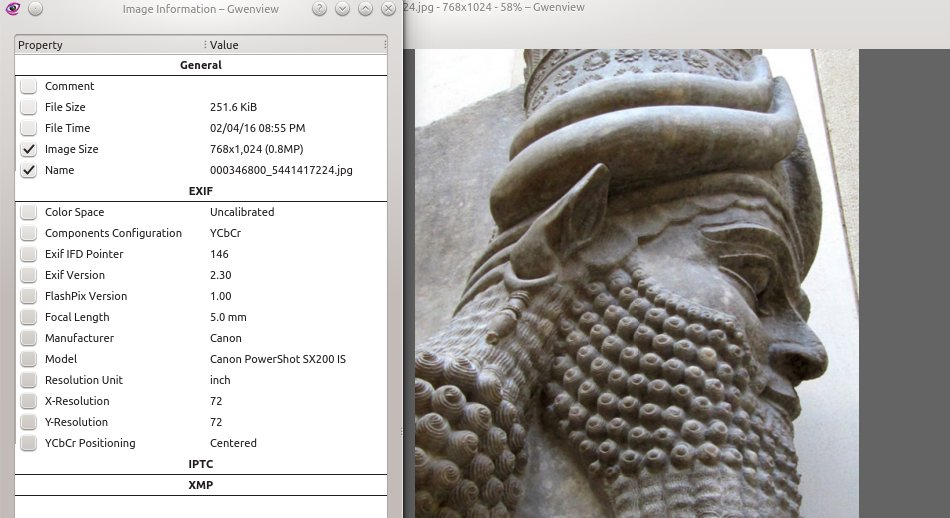
\includegraphics{mysnap78.jpg}}
\caption{exemple de donnes Exif accessibles}{\small 
image prise par un appareil Canon Powershot SX200 / focale de 5 mm
}\end{figure}

Pour manipuler les EXIFs de manière automatique nous utilisons le module Perl Image::ExifTool ainsi que la librairie Imagick et son module Perl Image::Magick pour un accès plus général aux opérations sur des images en ligne de commandes.

Grace a ces outils nous avons mis au point une suite de scripts permettant de classifier les images par données Exifs , taille de capteur , résolution etc .. de manière automatique.


\subsection{\textbf{Taille des capteurs CMOS}}
\label{collection:taille-des-capteurs-cmos}
Pour récupérer les informations de taille de capteur CMOS nous avons construit une base de données contenant plusieurs milliers de références d'appareils photos.Cette base de données est remise a jour si besoin a partir d'internet et notamment du site DPreview.com qui constitue la référence en la matière.
\begin{figure}[htbp]
\centering
\capstart

\scalebox{0.800000}{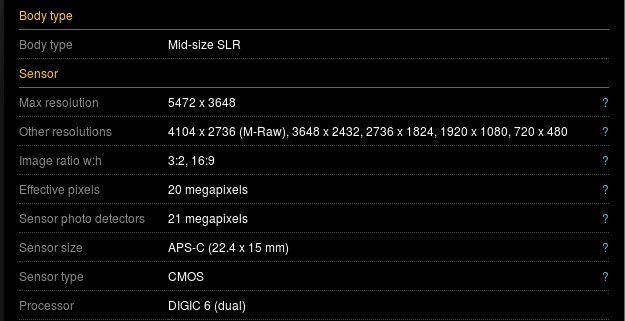
\includegraphics{mysnap80.jpg}}
\caption{exemple d'informations retournées par le site DPreview.com}{\small 
la taille du capteur est de 22.4 mm par 15 mm
}\end{figure}


\section{Structure From Motion}
\label{Sfm:structure-from-motion}\label{Sfm::doc}
La reconstruction 3D à partir d'images, image-based 3D reconstruction en anglais, désigne la technique qui permet d'obtenir une représentation en trois dimensions d'un objet ou d'une scène à partir d'un ensemble d'images prises sous différents points de vue de l'objet ou de la scène.

D'une manière plus générale, le problème appelé reconstruction 3D est le suivant : on dispose d'une ou plusieurs représentations en 2D d'un objet et on souhaite déterminer les coordonnées des éléments visibles sur ces représentations dans un repère de l'espace réel 3D.

il existe plusieurs logiciels permettant de faire cette reconstruction.


\subsection{\textbf{Logiciels OpenSource (libre)}}
\label{Sfm:logiciels-opensource-libre}\begin{itemize}
\item {} 
openMVG :  \href{http://imagine.enpc.fr/~moulonp/openMVG/}{http://imagine.enpc.fr/\textasciitilde{}moulonp/openMVG/}

\item {} 
TheiaSfm : \href{http://www.theia-sfm.org/}{http://www.theia-sfm.org/}

\item {} 
MVE : \href{http://www.gcc.tu-darmstadt.de/home/proj/mve/}{http://www.gcc.tu-darmstadt.de/home/proj/mve/}

\item {} 
bundler : \href{http://www.cs.cornell.edu/~snavely/bundler/}{http://www.cs.cornell.edu/\textasciitilde{}snavely/bundler/}

\end{itemize}


\subsection{\textbf{Logiciels commerciaux}}
\label{Sfm:logiciels-commerciaux}\begin{itemize}
\item {} 
Agisoft Photoscan : \href{http://www.agisoft.com/}{http://www.agisoft.com/}

\item {} 
Capturing Reality : \href{https://www.capturingreality.com/}{https://www.capturingreality.com/}

\item {} 
Autodesk 123D Catch : \href{http://www.123dapp.com/catch}{http://www.123dapp.com/catch}

\end{itemize}

\begin{DUlineblock}{0em}
\item[] La première étape consiste a séparer les images pour lesquelles nous disposons des données de focales et taille du capteur et celles ou ces données sont manquantes.
\item[] Une première passe nous permet de choisir automatiquement la paire d'images qui va permettre d'initialiser le processus incrémental de reconstruction.
\item[] Dans une seconde passe nous introduisons alors toutes les photos collectées et la paire d'images sélectionnées précédemment.
\end{DUlineblock}


\subsection{\textbf{Étapes de reconstruction}}
\label{Sfm:etapes-de-reconstruction}
-Extraction des points significatifs dans les images (Features).Il existe plusieurs types de descripteur pour cela (SIFT,A-KAZE).les descripteurs de type A-Kaze permettent de trouver plus de correspondances.
\begin{figure}[htbp]
\centering
\capstart

\scalebox{0.800000}{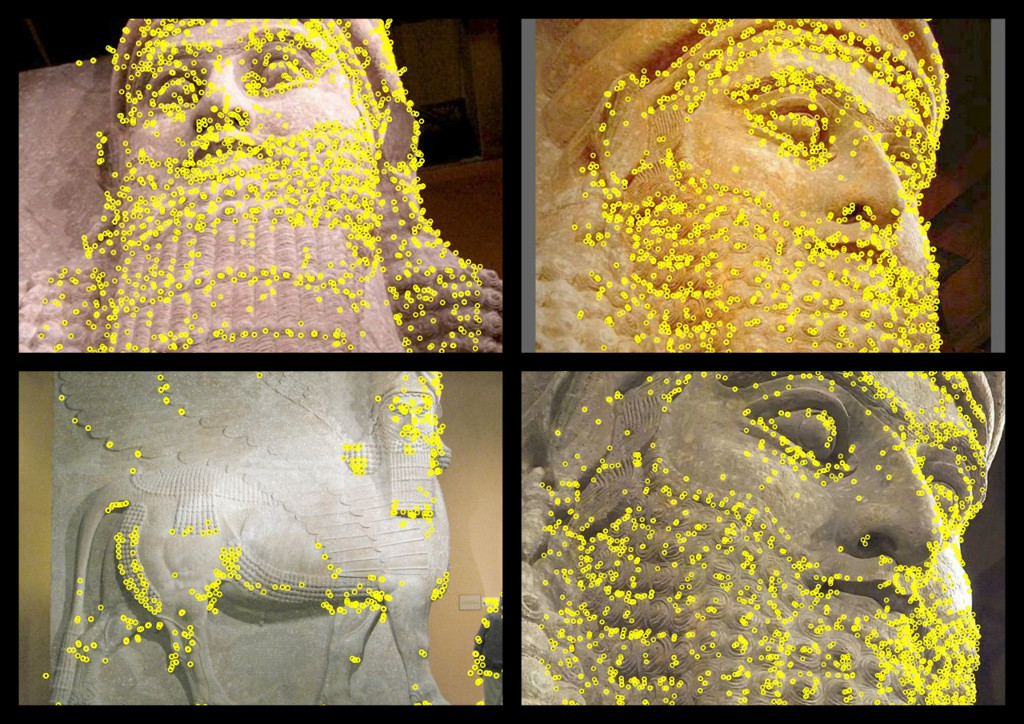
\includegraphics{features.jpg}}
\caption{exemple de features de type A-Kaze obtenues apres analyse des images}\end{figure}

-Recherches des correspondances entre toutes les features pour toutes les images traitées.(fig. 5)

-Reconstruction incrémentale des paramètres extrinsèques et intrinsèques de la camera (bundler adjustment)

-Une dernière passe peut être faite pour éliminer les points non robustes (robust estimation)

-On obtient alors une scène 3D contenant toutes les cameras reconstruites ainsi qu'un nuage de points décrivant de façon sommaire l'objet.(fig. 6)
\begin{figure}[htbp]
\centering
\capstart

\scalebox{1.000000}{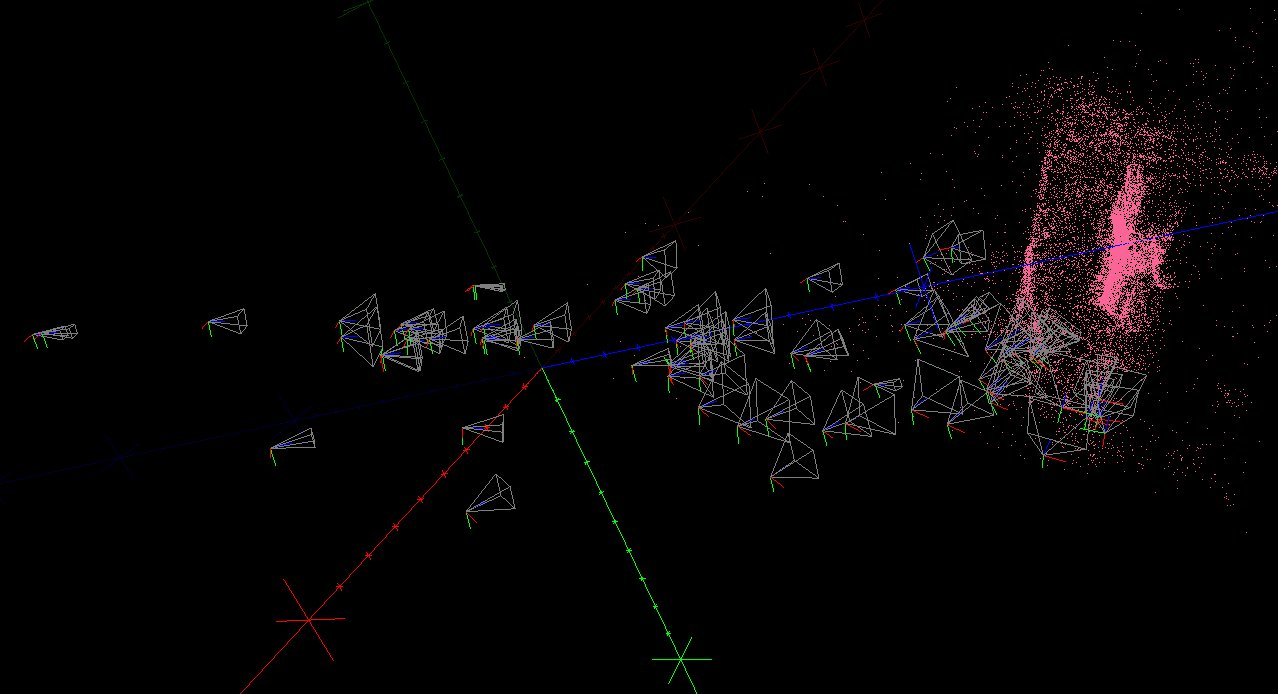
\includegraphics{mysnap20.jpg}}
\caption{exemple de scène obtenue aprés reconstruction incrémentale}{\small 
ici dans UMVE
}\end{figure}
\begin{figure}[htbp]
\centering
\capstart

\scalebox{0.800000}{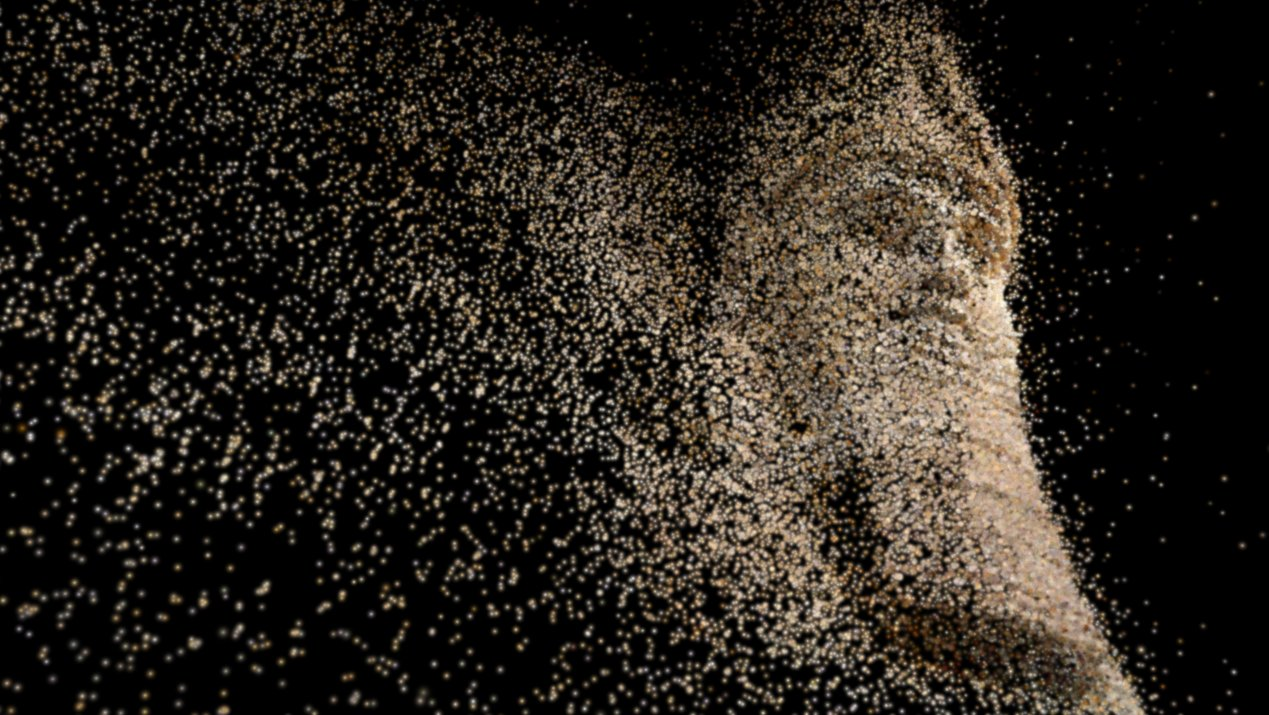
\includegraphics{mysnap8.jpg}}
\caption{exemple de nuage de points obtenu aprés reconstruction incrémentale}{\small 
\textasciitilde{}20000 points
}\end{figure}


\section{Multi-View Stereo}
\label{mvs:multi-view-stereo}\label{mvs::doc}
Cette étape correspond a la densification des données calculées précédemment. En exploitant les correspondances entre chaque image on va reconstituer un nuage de points beaucoup plus dense (plusieurs millions de points).Ces données sont stockées dans des maps de profondeur (depth map) puis recombinées dans un seul nuage de points. Enfin un maillage polygonal est généré a partir des points.

il existe plusieurs logiciels permettant de faire cette densification.


\subsection{\textbf{Logiciels OpenSource (libre)}}
\label{mvs:logiciels-opensource-libre}\begin{itemize}
\item {} 
openMVS :  \href{http://cdcseacave.github.io/openMVS/}{http://cdcseacave.github.io/openMVS/}

\item {} 
MVE/fssrecon : \href{http://www.gcc.tu-darmstadt.de/media/gcc/papers/Goesele-2007-MVS.pdf}{http://www.gcc.tu-darmstadt.de/media/gcc/papers/Goesele-2007-MVS.pdf}

\item {} 
CMVS/PMVS : \href{http://www.di.ens.fr/pmvs/}{http://www.di.ens.fr/pmvs/}

\end{itemize}


\subsection{\textbf{Logiciels commerciaux}}
\label{mvs:logiciels-commerciaux}\begin{itemize}
\item {} 
Agisoft Photoscan : \href{http://www.agisoft.com/}{http://www.agisoft.com/}

\item {} 
Capturing Reality : \href{https://www.capturingreality.com/}{https://www.capturingreality.com/}

\item {} 
Autodesk 123D Catch : \href{http://www.123dapp.com/catch}{http://www.123dapp.com/catch}

\end{itemize}


\subsection{\textbf{Étapes de reconstruction}}
\label{mvs:etapes-de-reconstruction}\begin{figure}[htbp]
\centering
\capstart

\scalebox{1.000000}{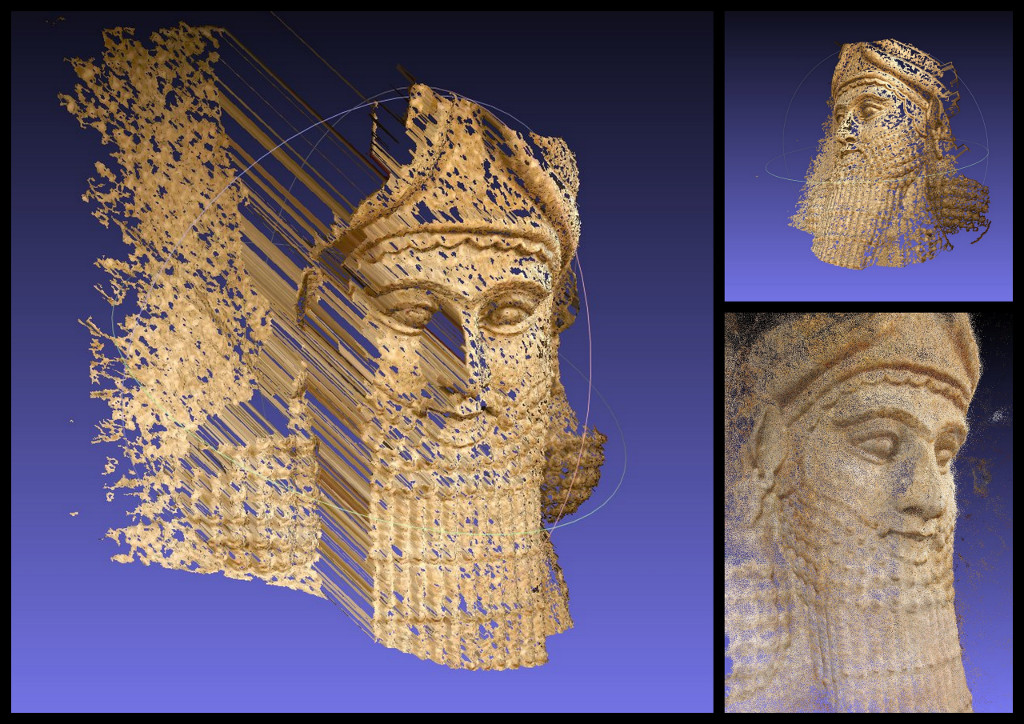
\includegraphics{mve3.jpg}}
\caption{depth map obtenue pour une image}{\small 
les points sont encore organisés en grille de pixels
}\end{figure}

Calcul des maps de profondeur (depth map).Le logiciel estime aussi une notion de qualité des points (confidence) ainsi que le gradient de profondeur dz indiquant des fortes variations de profondeur.(fig. 9)
\begin{figure}[htbp]
\centering
\capstart

\scalebox{1.000000}{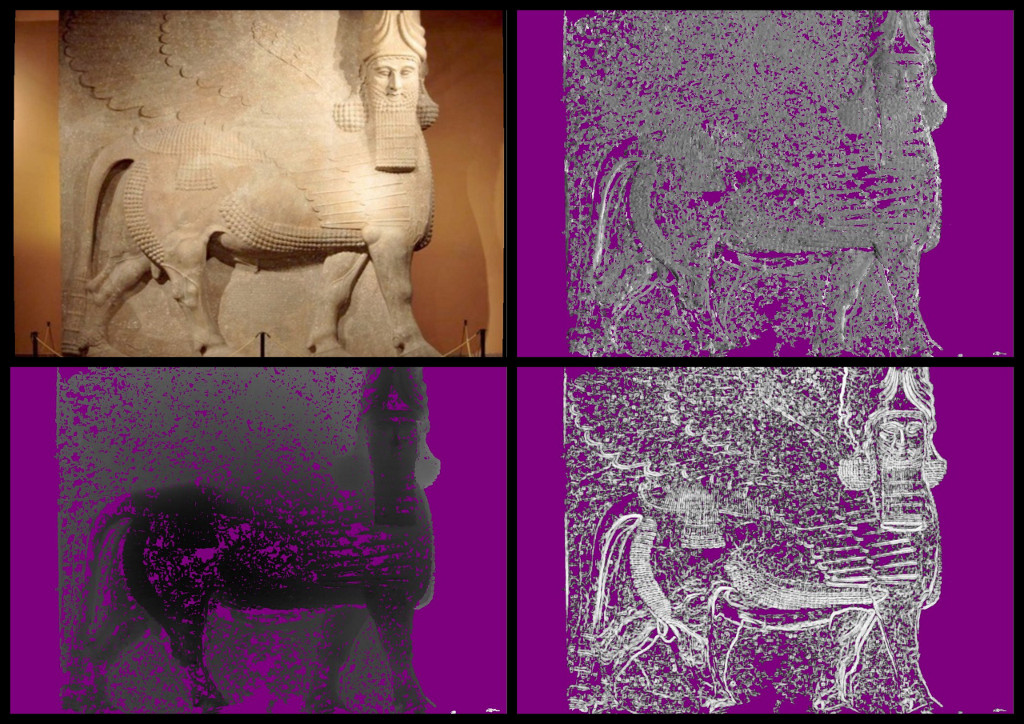
\includegraphics{mve2.jpg}}
\caption{visualisation d'une depth map (Umve)}{\small 
a) image originale b) dz
c) depth           e) confidence
}\end{figure}

Génération du nuage de points dense.(fig. 10 fig. 11)
\begin{figure}[htbp]
\centering
\capstart

\scalebox{0.800000}{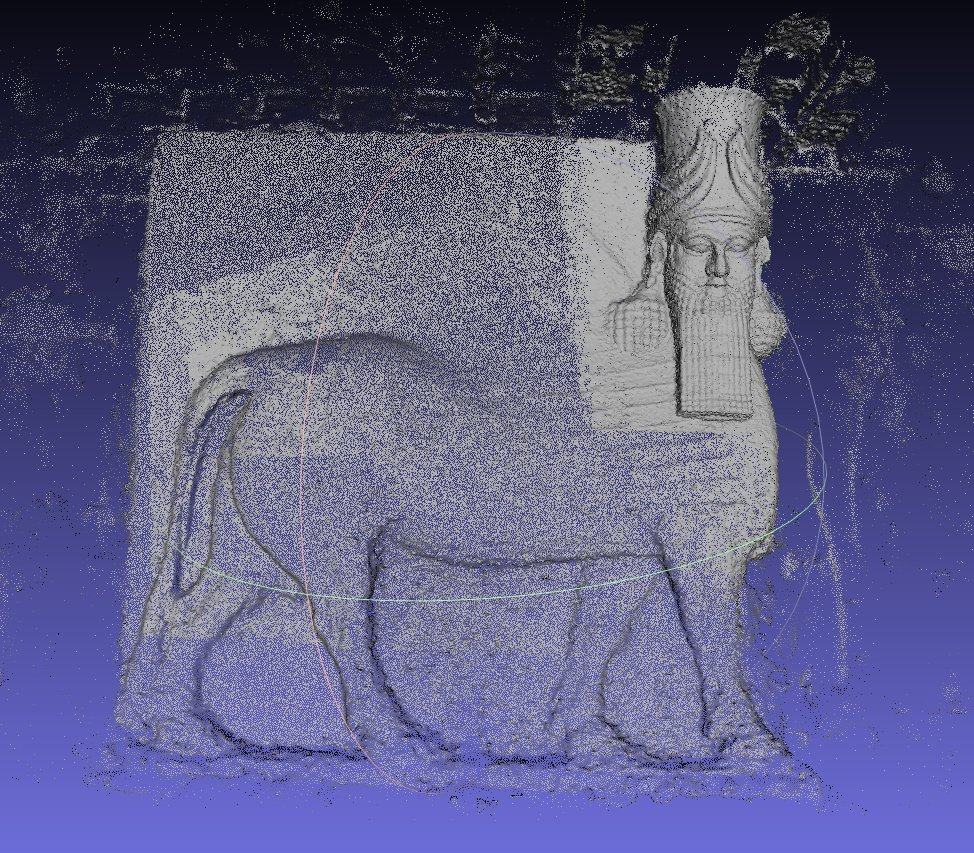
\includegraphics{mysnap12.jpg}}
\caption{dense point cloud}{\small 
plusieurs millions de points
}\end{figure}
\begin{figure}[htbp]
\centering
\capstart

\scalebox{0.800000}{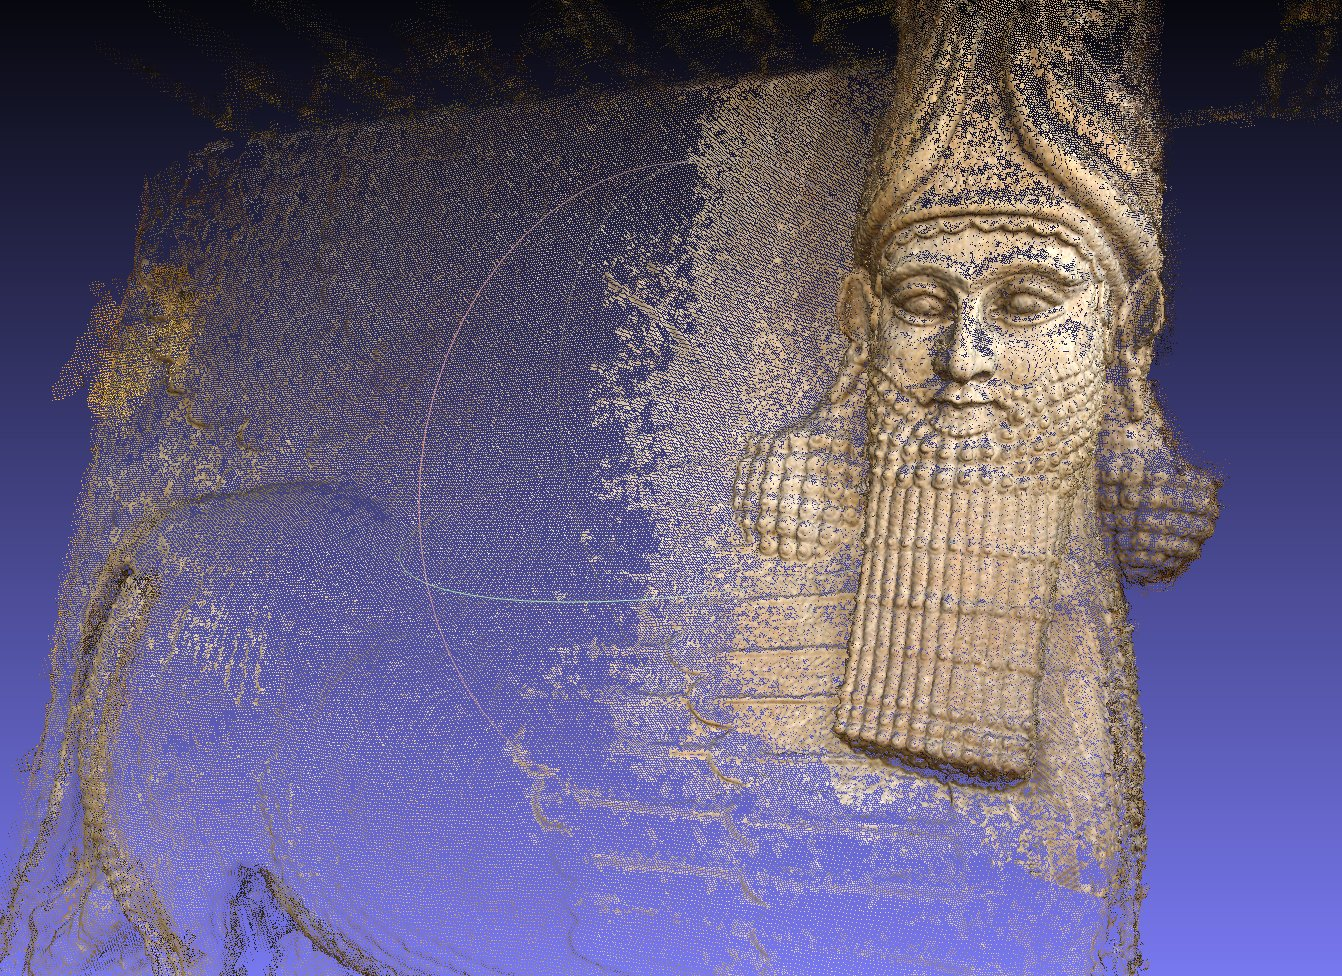
\includegraphics{mysnap18.jpg}}
\caption{dense point cloud}{\small 
plusieurs millions de points
}\end{figure}

Les points obtenus sont regroupes dans une structure de voxels (octree) puis filtrées et maillées pour générer un premier maillage polygonal,
ce maillage polygonal est alors raffiné avec divers algorithmes.(fig. 12)
\begin{figure}[htbp]
\centering
\capstart

\scalebox{0.800000}{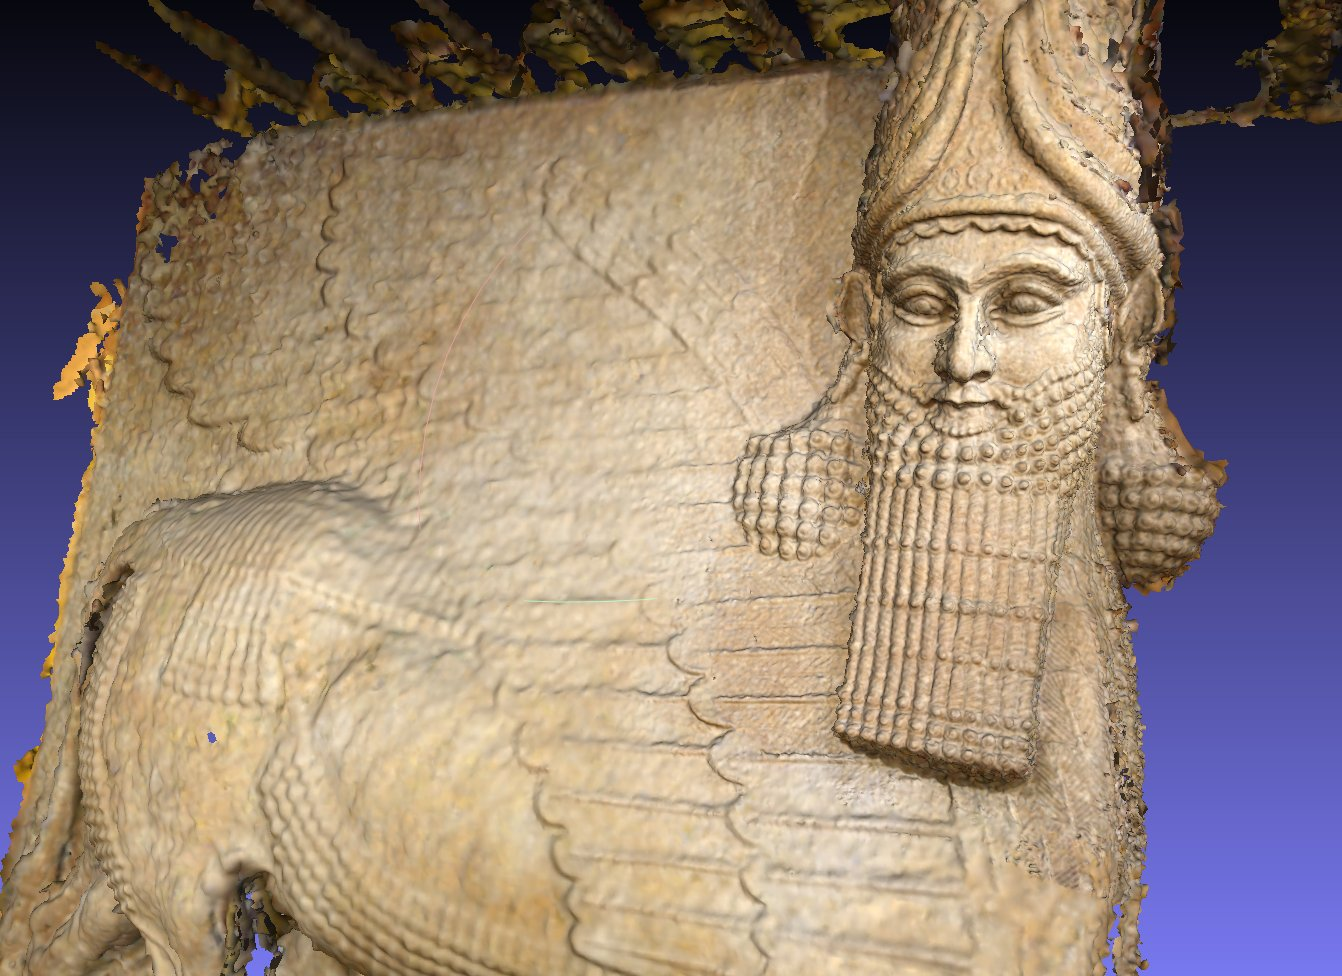
\includegraphics{mysnap19.jpg}}
\caption{exemple de maillage polygonal}{\small 
la couleur est appliquée uniquement aux points
}\end{figure}

Application de la texture.Une texture unique est générée en choisissant la meilleure vue dans toutes les photos et assemblée par une méthode de graph-cut au niveau des paramètres uv (atlas).(fig. 13)
\begin{figure}[htbp]
\centering
\capstart

\scalebox{0.800000}{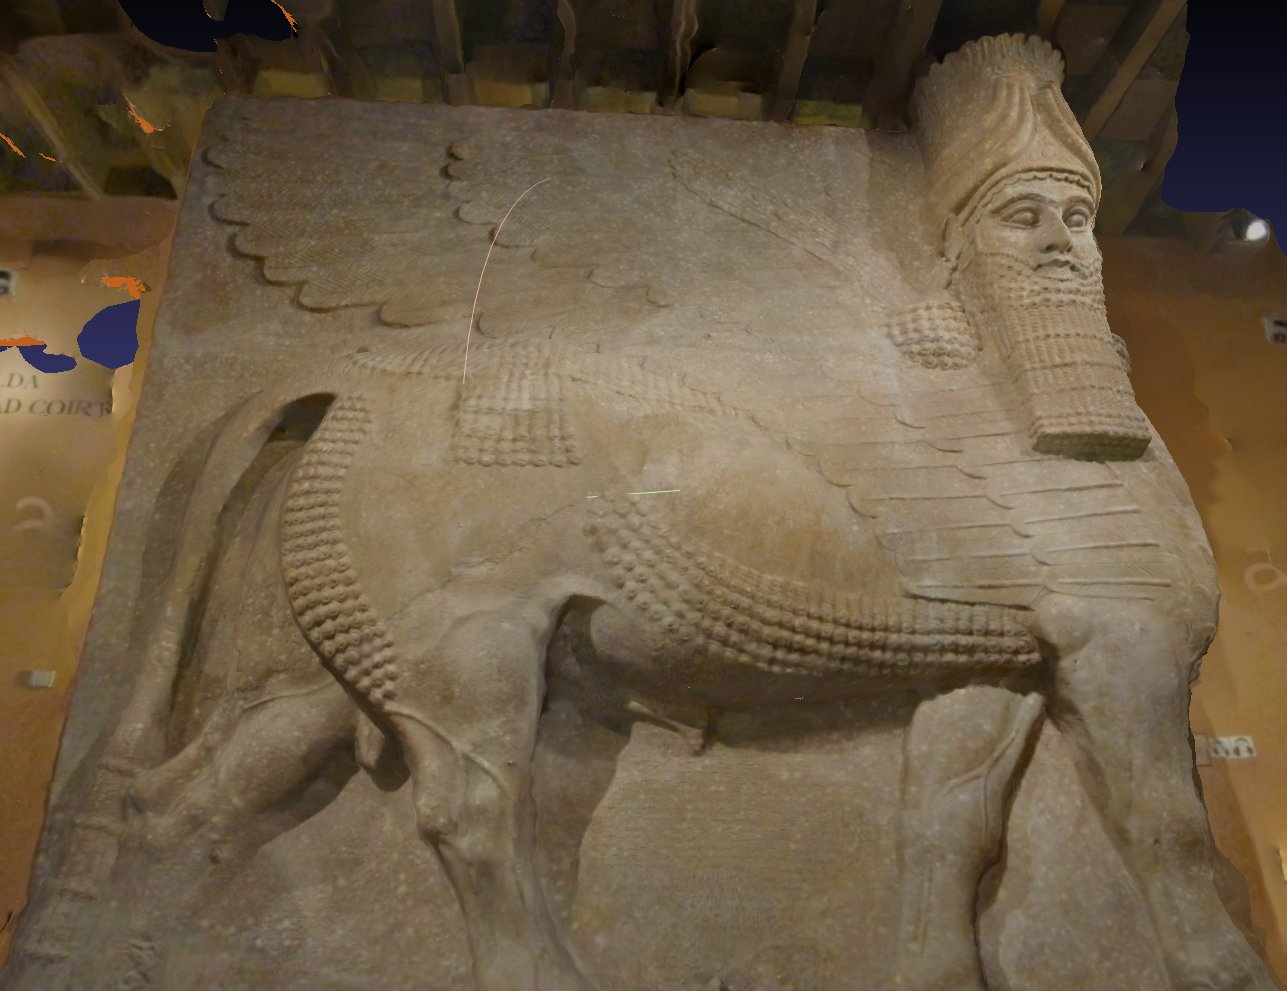
\includegraphics{mysnap17.jpg}}
\caption{le meme maillage avec sa texture appliquée}\end{figure}

Cette texture exploite le maximum de résolution fournie.Elle est par contre inexploitable dans un logiciel de retouche d'images (Photoshop ou Gimp).(fig. 14)
\begin{figure}[htbp]
\centering
\capstart

\scalebox{0.800000}{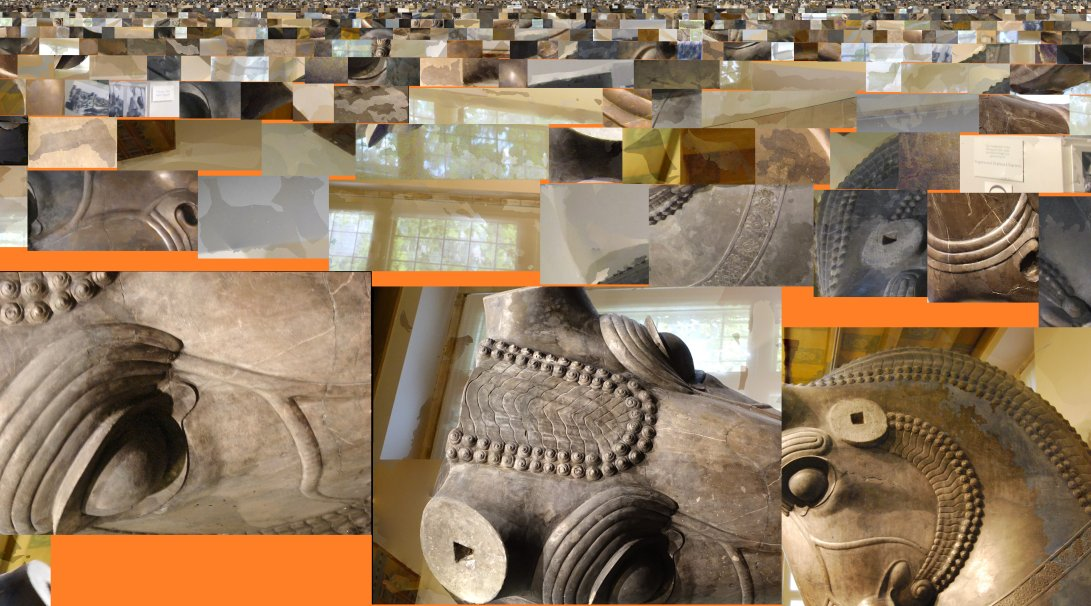
\includegraphics{mysnap50.jpg}}
\caption{exemple de texture (png) obtenue aprés projection}\end{figure}


\section{Finalisation}
\label{finalisation:finalisation}\label{finalisation::doc}
Une fois toutes ces étapes achevées , le modèle est exporté dans le logiciel Zbrush (Pixologic) ou les retouches finales seront faites par un artiste 3D.
\begin{figure}[htbp]
\centering
\capstart

\scalebox{1.000000}{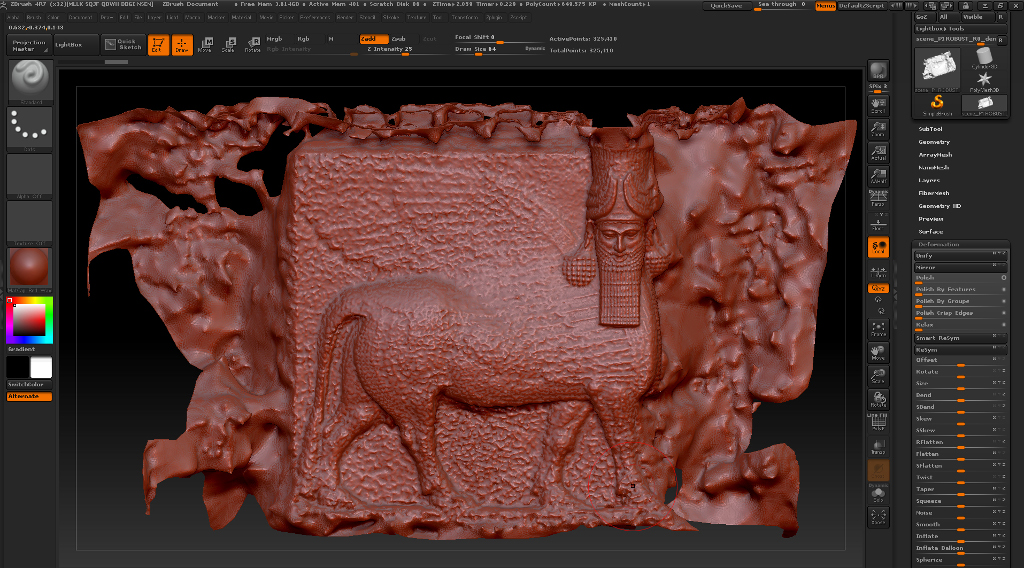
\includegraphics{zbrush1.jpg}}
\caption{resultat de la reconstruction avant retouche}{\small 
logiciel Zbrush - Pixologic
}\end{figure}

Ce logiciel permet de sculpter , a l'aide de différents outils , un objet 3d.On commence par supprimer toutes les parties inutiles du modèle puis a retoucher les parties mal reconstruites ou pas assez définies.
\begin{figure}[htbp]
\centering
\capstart

\scalebox{1.000000}{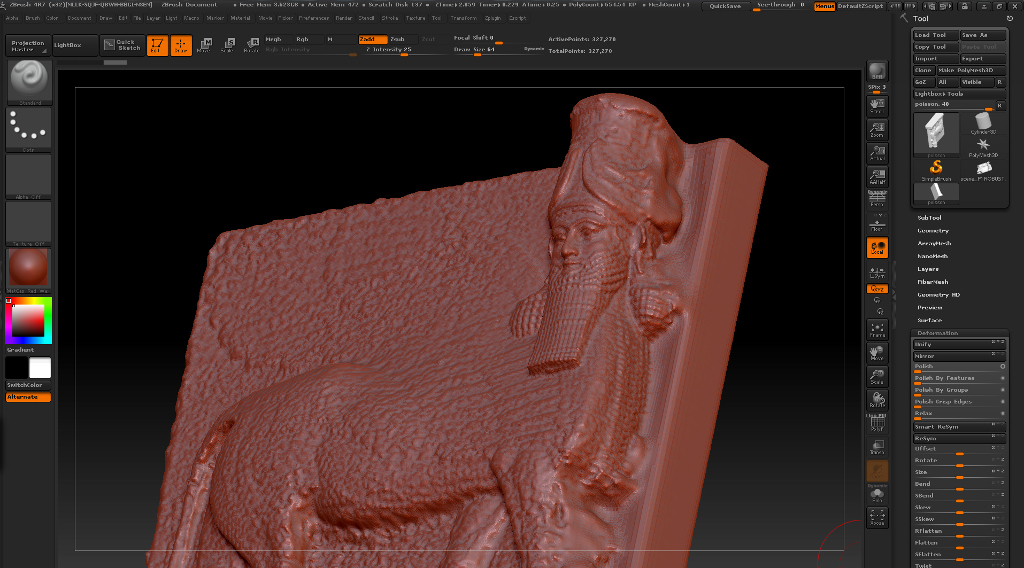
\includegraphics{zbrush3.jpg}}
\caption{resultat de la reconstruction en cours de retouche}{\small 
logiciel Zbrush - Pixologic
}\end{figure}

Zbrush permet aussi de diminuer considérablement le nombre de polygones et de générer des maps de displacement afin de rendre l'objet plus facilement manipulable dans les logiciels 3D utilises pour l'animation.

Ces maps de displacement permettent de retrouver tout les détails lors du calcul 3D dans un moteur de rendu au moment de la génération des images finales.


\section{Autres exemples}
\label{autres:autres-exemples}\label{autres::doc}
Colossal Bull Head from Persepolis - Musée oriental de Chicago.(fig. 15)

Ces têtes colossales servaient de protecteur aux bâtiments importants.
\begin{figure}[htbp]
\centering
\capstart

\scalebox{0.900000}{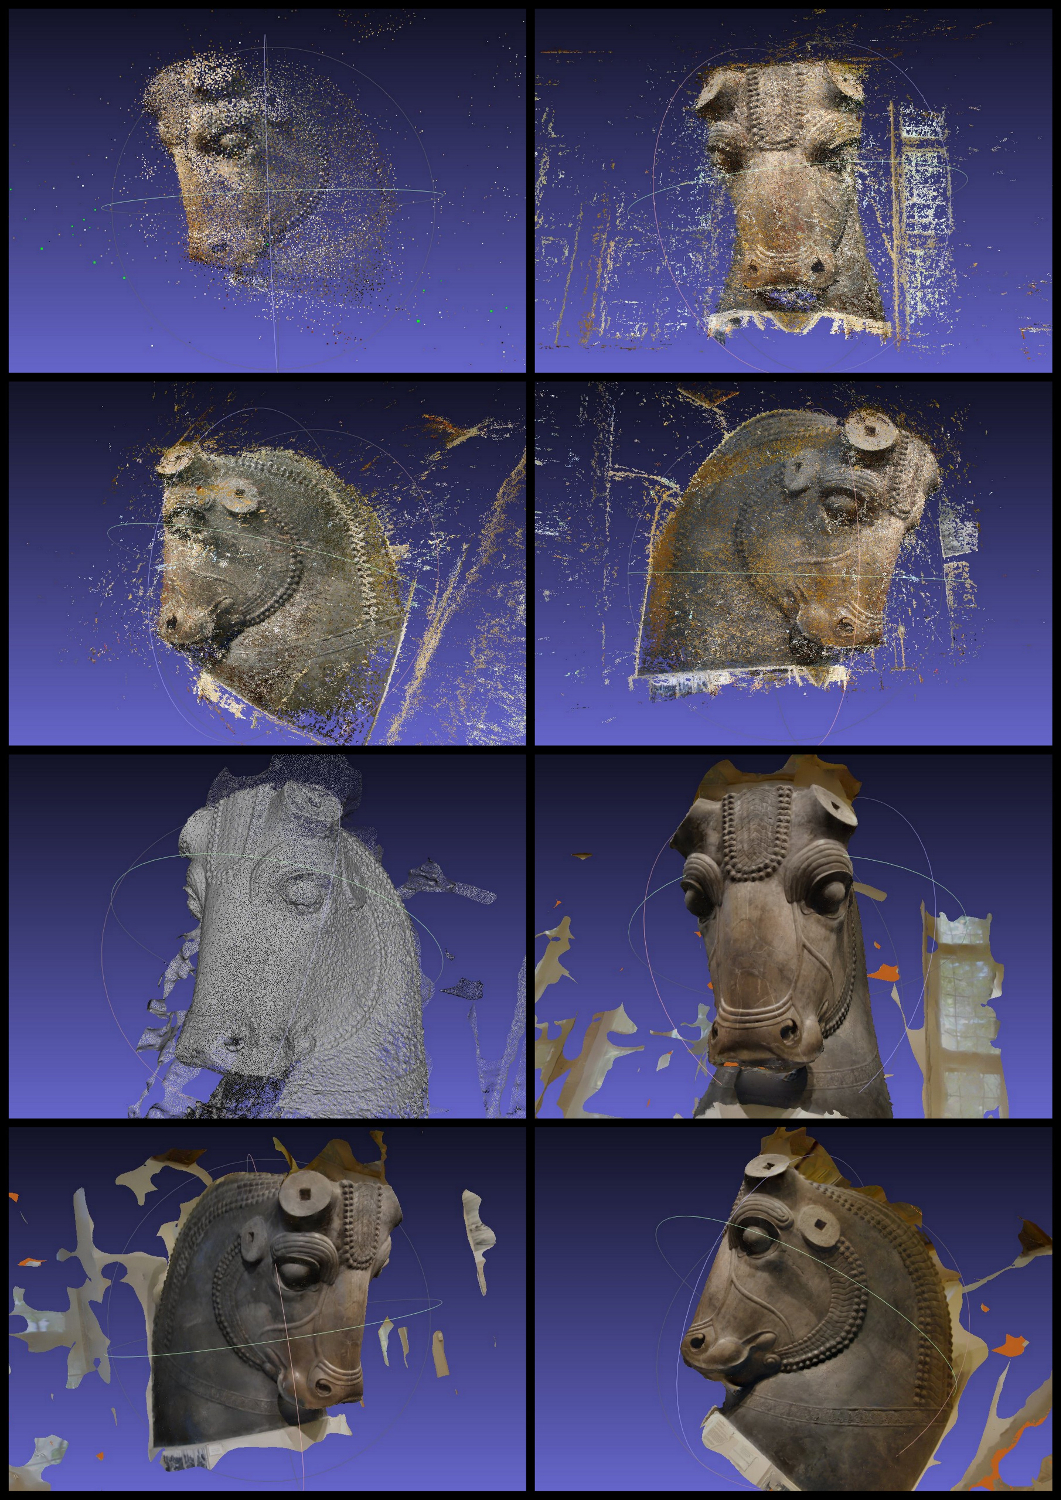
\includegraphics{bull.jpg}}
\caption{Colossal Bull Head from Persepolis - Musée oriental de Chicago}{\small 
reconstruction a partir de 73 photos collectées sur Internet
}\end{figure}



\renewcommand{\indexname}{Index}
\printindex
\end{document}
